\documentclass[fleqn]{article}
\oddsidemargin 0.0in
\textwidth 6.0in
\thispagestyle{empty}
\usepackage{import}
\usepackage{amsmath}
\usepackage{graphicx}
\usepackage{flexisym}
\usepackage{calligra}
\usepackage{amssymb}
\usepackage{bigints} 
\usepackage[english]{babel}
\usepackage[utf8x]{inputenc}
\usepackage{float}
\usepackage[colorinlistoftodos]{todonotes}


\DeclareMathAlphabet{\mathcalligra}{T1}{calligra}{m}{n}
\DeclareFontShape{T1}{calligra}{m}{n}{<->s*[2.2]callig15}{}
\newcommand{\scriptr}{\mathcalligra{r}\,}
\newcommand{\boldscriptr}{\pmb{\mathcalligra{r}}\,}

\definecolor{hwColor}{HTML}{442020}

\begin{document}

  \begin{titlepage}

    \newcommand{\HRule}{\rule{\linewidth}{0.5mm}}

    \center

    \begin{center}
      
\includegraphics[height=11cm, width=11cm]{asu.png}
    \end{center}

    \vline

    \textsc{\LARGE Statistical/Thermal Physics}\\[1.5cm]

    \HRule \\[0.5cm]
    { \huge \bfseries Quiz 8}\\[0.4cm] 
    \HRule \\[1.0cm]

    \textbf{Behnam Amiri}

    \bigbreak

    \textbf{Prof: Michael Treacy}

    \bigbreak

    \textbf{{\large \today}\\[2cm]}

    \vfill

  \end{titlepage}

  By signing my name, I am promising that I did this quiz on my own without any outside help.

  \vspace{0.5cm}

  Name: \textbf{Behnam Amiri}

  \vspace{1cm}
  
  \begin{center}
    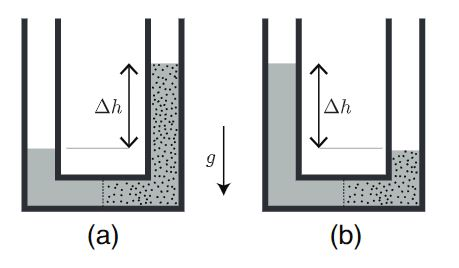
\includegraphics[height=7cm, width=10cm]{1.JPG}
  \end{center}

  Consider $n$ moles of a completely miscible mixture of two gases, $A$ and $B$, starting at temperature
  $T_P$. There are $(1-x)n$ moles of $A$ and $xn$ moles of $B$, giving an overall composition $A_{1-x} B_x$, with
  $0\leq x \leq  1$. The gas is cooled until it reaches temperature $T_{cd}$ (see diagram above), whereupon a
  small amount of liquid at composition d appears. Upon further cooling to temperature $T_{ab}$, the
  liquid fraction, $f$, increases, and the composition of the liquid follows the lower phase boundary
  line to point $b$ where the liquid composition is $A_{1-x_b} {B_x}_b$. Similarly, the gas phase follows
  the upper phase boundary line to point $a$, with gas composition $A_{1-x_a} {B_x}_a$. The fraction 
  of material that is gas is therefore $1-f$.

  \begin{enumerate}
    \item \textbf{(10 points)} As the system continues to cool, at what temperature does the system become
    $100\%$ liquid, (i.e. at which temperature is $f=1$)? Explain your reasoning.

      \textcolor{hwColor}{
        \\
        Basically, a \textbf{Temperature-composition} phase diagram is pretty much similar a pressure-composition
        diagram, except that the bubble and dew points are switched. Above the lense shaped graph, we have Gas and
        below it we have liquid and in the lens region, gas and liquid exist simultaneously 
        (which is very interesting to me).
        \\
        \\
        The boiling points are $T_A$ and $T_B$. At temperatures greater than $T_B$ the stable is a gas regardless of
        composition. As the temperature drops, free energy functions increases, $\dfrac{\partial G}{\partial T}=-S$,
        but for the gas is more because it has more entropy. At intermediate temperatures, between $T_A$ and $T_B$,
        either the liquid or the gas phase may be more stable.
        \\
        \\
        As it was explained in the question $\begin{cases}
          \text{Liquid fraction: } f 
          \\
          \text{Gas fraction: } 1-f 
        \end{cases}$. Upon cooling to temperature $T_{ab}$, $f$ increases simply because upon cooling, more amount 
        of gas condences. As we lowering the temperature, the gas $B$ concentration decreases in the liquid 
        descreases, but the gas $A$ starts to get more pure. and as we keep going down until we reach $T_{ef}$, 
        the average compostion \emph{must} always remain steadily on the line. Therefore, at $T_{ef}$, we have 
        $100\%$ liquid and $0\%$ gas.
        \\
      }
         
    \item \textbf{(20 points)} Keeping in mind that the total amount of $A$ and the total amount of $B$ 
    are invariant, derive an expression for the liquid fraction, $f$, at temperature $T_{ab}$. Show your work
    and explain clearly.

      \textcolor{hwColor}{
        \\
        This is where we can use the lever rule to come up with an expression for the liquid fraction. 
        We already have some horizontal lines on the graph helping us to derive an expression. Let's pick $T_{ab}$ 
        as our horizontal line and divide the line into two segments. (Left and right). The left part represents the portion liquid and the other
        side represents the portion of gas. Hence, the ratio of liquid to gas can be written as:
        \\
        \\
        $
          \begin{cases}
            \text{Length of the left horizontal line:} L.H.S: ~ x-x_a
            \\
            \\
            \text{Length of the right horizontal line:} L.H.S: ~ x_b-x
          \end{cases}
          \\
          \\
          \\
          \therefore ~~~ \boxed{
            R=\dfrac{x-x_a}{x_b-x} 
          } ~~~~ \checkmark
        $ 
      }

  \end{enumerate}

\end{document}
